 \begin{sloppypar}
\chapter{Applicazione Realizzata}
\fontsize{12}{19}\selectfont{Questo capitolo ha lo scopo di descrivere ed analizzare l’applicazione sviluppata per questo lavoro di tesi per il training di pazienti affetti da disturbi dello spettro autistico (DSA) e caratterizzata dalle potenzialità e risorse offerte dalle tecnologie introdotte nel capitolo precedente.\newline
In particolare, per \textit{training} si intende un insieme di attività volte al potenziamento delle abilità cognitive di un individuo\cite{Numero14}. Esse richiedono un serio e attento processo multidisciplinare che coinvolge diversi professionisti del settore medico e terapeutico, il cui obiettivo principale è valutare le abilità cognitive, comportamentali e sociali dei pazienti al fine di fornire una diagnosi accurata e un piano di trattamento personalizzato.\newline Inizialmente viene effettuata una valutazione da un team di specialisti che includono psicologi, psichiatri, neuropsichiatri infantili e terapisti occupazionali. Questa fase permette di raccogliere informazioni dettagliate sullo sviluppo del paziente, le sue abilità cognitive, il linguaggio, il comportamento sociale e le competenze motorie.\newline Sulla base delle informazioni raccolte nella valutazione iniziale, vengono selezionati i test più appropriati da sottoporre al paziente.\newline Questi test possono includere valutazioni standardizzate che misurano le abilità cognitive, il linguaggio, le abilità sociali e il comportamento adattivo dell'individuo.\newline

Nello specifico sono stati realizzati ed implementati due test molto diffusi per il training di pazienti affetti da DSA:
\begin{itemize}
\vspace{0.7cm}
    \item \textbf{Test sulla Discriminazione uditiva}\newline
    Il test sulla discriminazione uditiva è un test per l’analisi  delle funzioni linguistiche del paziente;
\vspace{1.2cm}
    \item \textbf{Test della Torre di Londra (TOL)}\newline
    Il Test della Torre di Londra (TOL) è un test per l’analisi delle funzioni esecutive del paziente.
\end{itemize}
\begin{figure}[H]
\centering
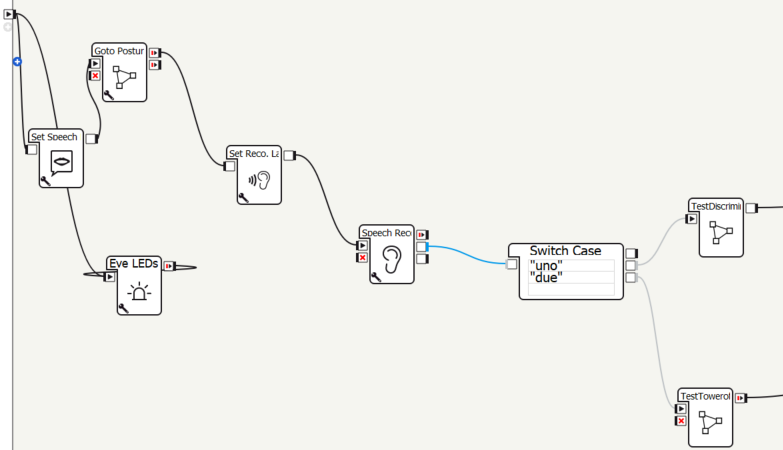
\includegraphics[width=1\textwidth]{immagini/applicazione.png}
\caption{Panoramica dell' applicazione realizzata tramite  il software Choregraphe}
\end{figure}
}

\newpage
\section{Discriminazione uditiva}
\fontsize{12}{19}\selectfont{La discriminazione uditiva è la capacità di percepire e riconoscere, attraverso
l’udito, le caratteristiche che rendono diversi fra loro i suoni della propria lingua, e
di attribuire ad essi un significato. Infatti, ogni fonema (ovvero ogni suono della
lingua) si differenzia dagli altri per una o più caratteristiche, definite “tratti”.\newline
Molte condizioni, tra cui l’autismo, possono influenzare l’abilità dell’individuo di
ascoltare e capire ciò che sente, ossia di comprendere, confrontare e distinguere i
“suoni” del linguaggio parlato.\newline Il Test sulla Discriminazione uditiva di \textit{Pinton}
e \textit{Zanettin} (1998) è utilizzato per valutare le abilità uditive e di elaborazione del
suono in individui con disturbi dello spettro autistico.
Nel caso particolare questo test è stato adoperato per valutare la capacità
uditiva dell’individuo di distinguere tra coppie di \textit{non parole}.\newline
La prova è composta
da 37 item, ciascuno dei quali rappresenta una coppia di non parole da
discriminare. Per ogni coppia vengono comunicate le non parole al paziente, il quale ha il compito di riconoscere se queste risultano essere uguali o diverse tra loro.\newline
Nel caso in cui
la risposta fosse corretta, questo comporterebbe un aumento del punteggio del
paziente (definito \textit{score} e registrato per ogni paziente). Lo score di ogni paziente rappresenta
una metrica fondamentale per il terapista, il quale dopo averlo analizzato
può verificare la presenza di eventuali disturbi nelle funzionalità uditive del paziente.
}
\vspace{0.2cm}
\subsection{Implementazione}
\fontsize{12}{19}\selectfont{Per l’implementazione di questo test sono stati utilizzati diversi box script Python in Choregraphe, i quali verranno analizzati di seguito:
\vspace{0.4cm}
\begin{itemize}
    \item \textbf{Animated Say text}: box che consente a Pepper di emettere messaggi
vocali animati. Questo box integra le funzionalità di sintesi vocale del robot,
consentendogli di comunicare verbalmente con gli utenti in modo coinvolgente e
realistico. Riceve in input un box testuale e lo trasforma in un messaggio vocale
animato.
\vspace{0.3cm}
\begin{figure}[H]
\centering
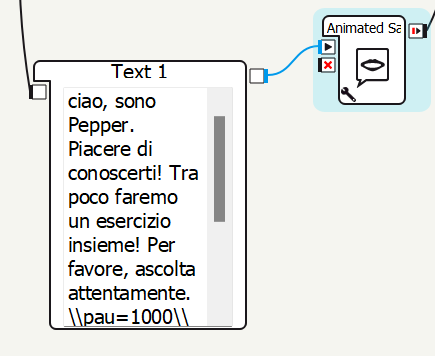
\includegraphics[width=0.5\textwidth]{immagini/Text.png}
\caption{Box per la lettura di testo animato}
\end{figure}
\vspace{0.3cm}
    \item \textbf{Record Sound}: box che permette di registrare i suoni catturati dai microfoni
direzionali di Pepper e salvarli sulla memoria temporanea di quest’ultimo.
\vspace{0.3cm}
\begin{figure}[H]
\centering
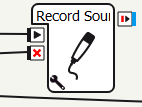
\includegraphics[width=0.23\textwidth]{immagini/RS.png}
\caption{Box per la registrazione audio}
\end{figure}
\vspace{0.3cm}    
    \item \textbf{Record Video}: box che permette di registrare video catturati dalle telecamere
frontali posizionate negli occhi di Pepper e salvarlo sulla memoria temporanea
di quest’ultimo.
\vspace{0.1cm}
\begin{figure}[H]
\centering
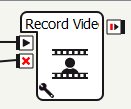
\includegraphics[width=0.23\textwidth]{immagini/RV.png}
\caption{Box per la registrazione video}
\end{figure}
\vspace{0.3cm}    
    \item \textbf{Face Tracker}: box progettato per rilevare e tracciare i volti umani
nell’ambiente circostante il robot. Questo modulo consente a Pepper di identificare
e seguire i volti umani, facilitando l’interazione e la comunicazione
con gli utenti. Questo modulo utilizza una combinazione di algoritmi di visione
artificiale e sensori per individuare i volti presenti nell’ambiente circostante.\newline L’immagine acquisita
viene quindi elaborata utilizzando algoritmi di elaborazione dell’immagine
per individuare le caratteristiche facciali comuni associate ai volti umani, come
gli occhi, il naso e la bocca. Questa elaborazione può includere tecniche come
la segmentazione dell’immagine, la rilevazione dei contorni e il riconoscimento
delle caratteristiche.\newline
Una volta individuato il volto, il modulo Face Tracker traccia
e segue i movimenti di quest’ ultimo nel tempo. Questo consente a Pepper
di mantenere una connessione visiva con le persone nell’ambiente e di rilevare
eventuali cambiamenti di posizione o espressione facciale. Il robot quindi può
mantenere il contatto visivo con una persona mentre si sposta o può indirizzare i
suoi movimenti e le sue espressioni facciali verso un individuo specifico per creare
una connessione personale.
\vspace{0.1cm}
\begin{figure}[H]
\centering
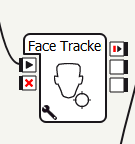
\includegraphics[width=0.23\textwidth]{immagini/FT.png}
\caption{Box per il tracciamento del volto umano}
\end{figure}
\vspace{0.3cm}      
    \item \textbf{Set Language}: box che permette di settare la lingua riconosciuta e parlata
del robot.
\vspace{0.1cm}
\begin{figure}[H]
\centering
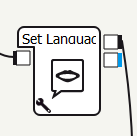
\includegraphics[width=0.23\textwidth]{immagini/Language.png}
\caption{Box per settare la lingua riconosciuta dal robot}
\end{figure}
\vspace{0.3cm}       
    \item \textbf{LRS} (lettura,riconoscimento vocale e incremento dello score): box che
racchiude uno script python personalizzato e che permette al robot di leggere le
coppie di non parole all’utente, aspettare la risposta di quest’ ultimo e verificarne
la correttezza. Nel caso in cui la risposta fosse corretta, verrebbe incrementato lo
score dell’utente, salvando il valore di quest’ ultimo in un file esterno.
\vspace{0.1cm}
\begin{figure}[H]
\centering
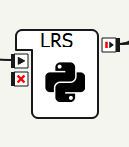
\includegraphics[width=0.23\textwidth]{immagini/LRS.png}
\caption{Box Python personalizzato}
\end{figure}
\vspace{0.3cm} 
\end{itemize}
Di seguito viene riportato e analizzato il codice dello script Python personalizzato denominato
LRS:
\begin{figure}[H]
\centering
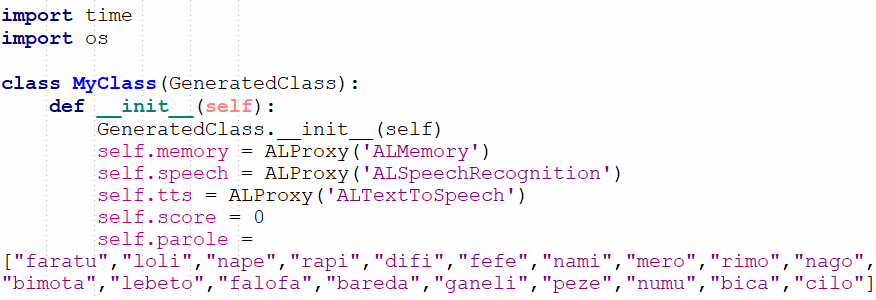
\includegraphics[width=1\textwidth]{immagini/lrs1.png}
\end{figure}
Alla creazione della classe vengono inizializzati gli oggetti che verranno utilizzati
per accedere alla memoria tramite modulo \textit{ALMemory}, al riconoscimento della
voce umana tramite modulo \textit{ALSpeechRecognition} e per la lettura vocale di un
testo tramite modulo \textit{ALTextToSpeech}. Fatto ciò viene inizializzata la lista delle
non parole che faranno parte del test.
\vspace{0.3cm}
\begin{figure}[H]
\centering
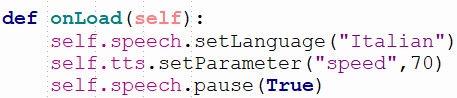
\includegraphics[width=0.7\textwidth]{immagini/lrs2.png}
\end{figure}
\vspace{0.3cm}
La funzione \textit{onLoad} viene invocata al caricamento del box e permette di inizializzare
alcuni parametri del robot. Viene impostata la lingua del componente
di sintesi vocale (\textit{self.speech}) su italiano e viene settato il parametro di velocità
(\textit{speed}) del componente di sintesi vocale (\textit{self.tts}) che rappresenta la velocità di
lettura di un testo di Pepper.
\vspace{0.3cm}
\begin{figure}[H]
\centering
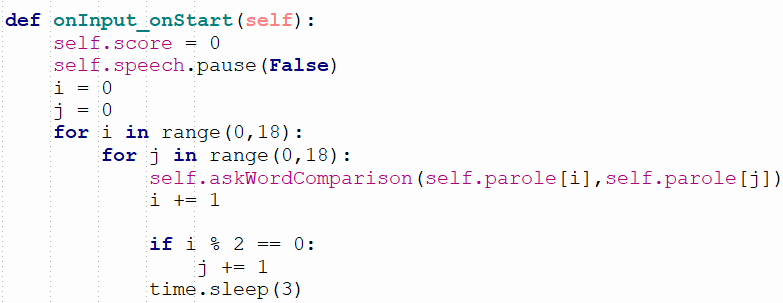
\includegraphics[width=1.05\textwidth]{immagini/lrs3.png}
\end{figure}
\vspace{0.3cm}
La funzione \textit{onInput onStart} viene invocata quando il box riceve un input esterno.
In particolare il funzionamento di questa porzione di codice viene descritto di
seguito.
\newline
Per prima cosa viene inizializzata a 0 una variabile \textit{score} che terrà traccia
del punteggio del paziente durante il test. Successivamente viene richiamata l’esecuzione del
componente di sintesi vocale e vengono inizializzati due indici, \textit{i} e \textit{j}, per riferirsi di
volta in volta a due non parole dalla lista di non parole inizializzata in precedenza.\newline
Il ciclo \textit{for} successivo permette di iterare, scorrendo la lista di non parole e creando
delle coppie da comunicare al paziente per lo svolgimento del test.\newline
A questo punto viene richiamata la funzione \textit{askWordComparison} il cui funzionamento
verrà analizzato successivamente. Al termine della funzione viene
utilizzato il metodo \textit{time.sleep()} per introdurre un ritardo di 3 secondi nel programma,
così da creare una pausa tra le iterazioni del ciclo.
\begin{figure}[H]
\centering
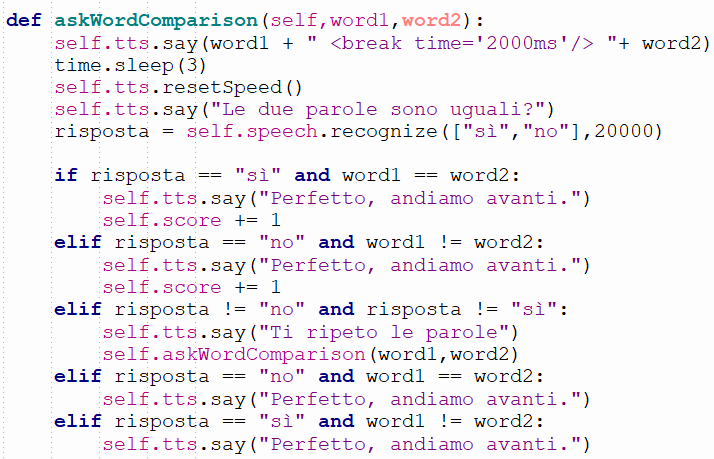
\includegraphics[width=1\textwidth]{immagini/lrs4.png}
\end{figure}
\vspace{0.3cm}
La funzione \textit{askWordComparison} prende in input due parole (\textit{word1} e \textit{word2}) e
svolge una serie di operazioni per confrontare la risposta del paziente, dopo averle
comunicate a quest’ultimo.\newline
Per prima cosa viene utilizzo il componente di sintesi vocale (\textit{self.tts}) per
riprodurre l’audio delle due non parole concatenate insieme, separandole da una pausa
di 2000 millisecondi (2 secondi). Viene utilizzato il metodo \textit{say} facendo si che
Pepper pronunci le due non parole, separate da una pausa per scandirle correttamente,
al paziente.\newline
Fatto ciò Pepper porrà una domanda al paziente, chiedendo se le due
non parole siano uguali e resterà in attesa di una sua risposta.\newline
Una volta ottenuta verrà analizzata per 5 casistiche:
\vspace{0.2cm}
\begin{enumerate}
    \item Se la risposta dell’utente è "\textbf{sì}" e le due parole sono \textbf{uguali}, viene incrementato
il punteggio del paziente in quanto la risposta risulta corretta e viene
pronunciato il messaggio "\textit{Perfetto, andiamo avanti.}"
\vspace{0.2cm}
\item Se la risposta dell’utente è "\textbf{no}" e le due parole sono \textbf{diverse}, viene incrementato
il punteggio del paziente in quanto la risposta risulta corretta e
viene pronunciato il messaggio "\textit{Perfetto, andiamo avanti.}"
\vspace{0.2cm}
\item Se la risposta dell’utente non è né "\textbf{no}" né "\textbf{sì}", viene pronunciato il messaggio
"\textit{Ti ripeto le parole}" e la funzione \textit{askWordComparison} viene richiamata nuovamente per ottenere una nuova risposta dall’utente.
\vspace{0.2cm}
\item Se la risposta dell’utente è "\textbf{no}" e le due parole sono \textbf{uguali}, non viene
incrementato il punteggio del paziente in quanto la risposta non è corretta
e viene pronunciato il messaggio "\textit{Perfetto, andiamo avanti.}"
\vspace{0.2cm}
\item Se la risposta dell’utente è "\textbf{sì}" e le due parole sono \textbf{diverse}, non viene
incrementato il punteggio del paziente in quanto la risposta non è corretta
e viene pronunciato il messaggio "\textit{Perfetto, andiamo avanti.}"
\end{enumerate}
\vspace{0.3cm}
\begin{figure}[H]
\centering
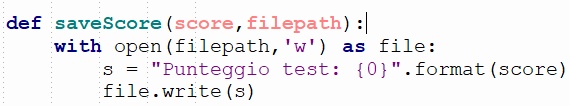
\includegraphics[width=0.8\textwidth]{immagini/lrs5.png}
\end{figure}
\vspace{0.3cm}
La funzione \textit{saveScore} accetta due argomenti: \textbf{score}, che rappresenta il punteggio
del paziente da salvare e \textbf{filepath}, che indica il percorso del file in cui il punteggio
verrà salvato.\newline
Più nello specifico, la funzione accede al file specificato dal \textbf{filepath} passato
come argomento, crea una stringa formattata che include il punteggio e scrive
questa stringa all’interno del file.
\vspace{0.3cm}
\begin{figure}[H]
\centering
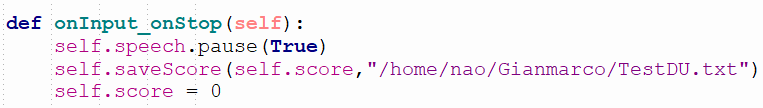
\includegraphics[width=1\textwidth]{immagini/lrs6.png}
\end{figure}
\vspace{0.3cm}
Al termine dello script viene invocata la procedura \textit{onInput onStop} che si occupa
di attivare l’output del box, di richiamare la funzione \textit{saveScore} per salvare il
punteggio del paziente su un file esterno e di inizializzare il valore della variabile
\textit{score} a 0.
}
\newpage




\section{Torre di Londra (ToL)}
\fontsize{12}{19}\selectfont{
Il Test della Torre di Londra (ToL) è un test cognitivo sviluppato negli anni
ottanta del secolo scorso da \textit{Tim Shallice} e \textit{Rosaleen A. McCarthy}. Esso è utilizzato
con bambini e adulti per misurare eventuali deficit cognitivi, che riducono la
capacità del soggetto di pianificare, mantenere l’attenzione, decidere e risolvere
problemi.\newline Non è specificamente rivolto ai disturbi dello spettro autistico (DSA),
ma può essere utilizzato per valutare le abilità cognitive di individui con DSA e
altre condizioni.
In particolare il test consiste in un supporto con tre paletti verticali di diverse
altezze e un insieme di palline colorate (\textcolor{Green}{verde}, \textcolor{red}{rosso} e \textcolor{blue}{blu}).
\vspace{0.6cm}
\begin{figure}[H]
\centering
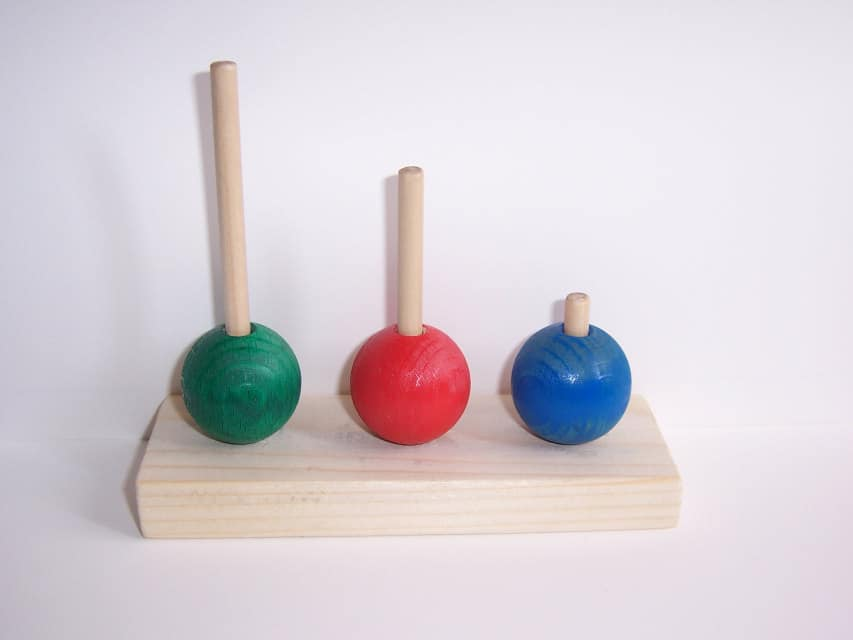
\includegraphics[width=0.45\textwidth]{immagini/TOL.png}
\caption{Supporto fisico utilizzato durante la somministrazione del test}
\end{figure}

L’obiettivo del test è spostare le palline da una configurazione iniziale a una
configurazione obiettivo, seguendo quattro regole:
\begin{enumerate}
    \item \textbf{Prima regola}: è possibile può spostare una sola pallina alla volta.
    \vspace{0.15cm}
    \item \textbf{Seconda regola}: si può muovere una sola pallina da un paletto ad un altro, in modo tale da non consentire all’utente di posizionare le palline sul tavolo o averne in mano più di una alla volta.
\vspace{0.4cm}
\item \textbf{Terza regola}: è possibile inserire una sola pallina sul paletto più
piccolo, due su quello intermedio e tre su quello più grande.
\vspace{0.4cm}
\item \textbf{Quarta regola}: bisogna attenersi al numero di spostamenti massimi consentiti
per risolvere il problema.
\end{enumerate}
\vspace{0.8cm}
Per poter calcolare il punteggio finale raggiunto dal paziente al termine del test, è
necessario tenere in considerazione il numero di problemi risolti correttamente, il
numero di mosse utilizzate per risolverli e la violazione delle regole
esplicitate precedentemente.\newline
Nel caso specifico dell’applicazione sviluppata, il test viene somministrato
dal robot Pepper attraverso i seguenti passi:
\begin{itemize}
    \item prima di iniziare il robot effettua un'introduzione al test e spiega le
regole fornendo un esempio pratico visualizzato sul suo tablet,
per assicurarsi che il paziente abbia compreso le istruzioni;
\vspace{0.4cm}
    \item dopo aver esplicitato le regole del test, il robot presenta la configurazione
iniziale del problema e la configurazione obiettivo;
\vspace{0.4cm}
    \item il paziente viene invitato da Pepper a risolvere il problema nel minor numero
possibile di mosse, senza limiti di tempo. Tuttavia, viene registrato il tempo
impiegato per completare il test a scopo diagnostico;
\vspace{0.4cm}
    \item l’esaminatore registra il numero di mosse utilizzate dal paziente, l’eventuale
violazione di regole e se il problema è stato risolto correttamente o meno;
\vspace{0.4cm}
    \item il test viene ripetuto per diverse configurazioni e nel caso specifico viene
ripetuto per 12 configurazioni con difficoltà crescente.
\end{itemize}

}
\newpage
\subsection{Implementazione}
\fontsize{12}{19}\selectfont{
Per l’implementazione di questo test sono stati utilizzati diversi
box script Python in Choregraphe, i quali verranno analizzati
di seguito:
\vspace{0.4cm}
\begin{enumerate}
    \item \textbf{Animated Say text, Record Sound, Record Video, Set language e
Face tracker}: già analizzati in precedenza.
\vspace{0.4cm}

\item \textbf{Show image}: box che permette di mostrare sul tablet di Pepper un’immagine
specifica, recuperata dalla memoria interna del robot.
\vspace{0.4cm}
\begin{figure}[H]
\centering
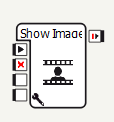
\includegraphics[width=0.2\textwidth]{immagini/si.png}
\end{figure}
\vspace{0.4cm}
\item \textbf{Set Recognition Language}: box che permette di settare la lingua riconosciuta
e compresa dal robot.
\vspace{0.4cm}
\begin{figure}[H]
\centering
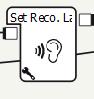
\includegraphics[width=0.18\textwidth]{immagini/srl.png}
\end{figure}
\vspace{0.4cm}
\item \textbf{Speech Recognition}: box di riconoscimento vocale che utilizza algoritmi
e modelli di riconoscimento vocale avanzati per interpretare il parlato degli
utenti.\newline Per prima cosa il box cattura l’input audio proveniente dal microfono
del robot o di un dispositivo esterno, come ad esempio un microfono
collegato al computer in cui è in esecuzione Choregraphe.\newline L’audio viene successivamente pre-elaborato
per migliorare la qualità del segnale e rimuovere eventuali rumori
di fondo indesiderati. Infine l’audio pre-elaborato viene inviato all’algoritmo
di riconoscimento vocale, che confronta il parlato con un modello linguistico
e/o una serie di modelli acustici per determinare il testo corrispondente.
\vspace{0.4cm}
\begin{figure}[H]
\centering
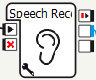
\includegraphics[width=0.18\textwidth]{immagini/sr.png}
\end{figure}
\vspace{0.4cm}
\item \textbf{Switch Case}: box che, dopo aver ricevuto la risposta dell’utente, stimola
un solo output tra quelli disponibili. Utilizzato in questo caso per proseguire
con la somministrazione del test, o ripetere le regole iniziali.
\vspace{0.4cm}
\begin{figure}[H]
\centering
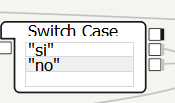
\includegraphics[width=0.27\textwidth]{immagini/sc.png}
\end{figure}
\vspace{0.4cm}
\item \textbf{Tablet touch}: box che invia un segnale nel momento in cui il tablet di
Pepper viene toccato da un utente.
\vspace{0.4cm}
\begin{figure}[H]
\centering
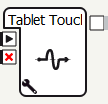
\includegraphics[width=0.18\textwidth]{immagini/tt.png}
\end{figure}
\vspace{0.4cm}
\item \textbf{Figure}: diagramma di box composto da molteplici box utilizzati per somministrare
il test ToL.
\vspace{0.4cm}
\begin{figure}[H]
\centering
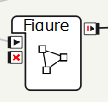
\includegraphics[width=0.2\textwidth]{immagini/figure.png}
\end{figure}
\vspace{0.4cm}
\end{enumerate}
Entrando nello specifico del box Tablet Touch questo presenta delle funzioni
python personalizzate:
\vspace{0.4cm}
\begin{itemize}
    \item \textbf{startTimer}: funzione che salva l’istante di inizio del test, per ogni figura,
in una variabile timer.
\vspace{0.6cm}
\begin{figure}[H]
\centering
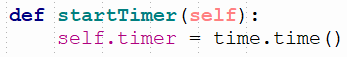
\includegraphics[width=0.6\textwidth]{immagini/starttimer.png}
\end{figure}
\vspace{0.6cm}
\item \textbf{stopTimer}: funzione che interrompe il timer e calcola la durata del tempo
trascorso dal momento in cui la figura è stata mostrata al paziente, al momento
in cui viene toccato il tablet del robot.
\vspace{0.6cm}
\begin{figure}[H]
\centering
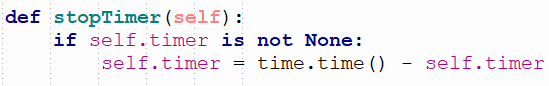
\includegraphics[width=0.8\textwidth]{immagini/stoptimer.png}
\end{figure}
\vspace{0.6cm}
\item \textbf{saveTimerValue}: funzione che, dopo aver recuperato il valore della variabile \textit{timer} (\textit{self.timer}), lo formatta in minuti e secondi.\newline Successivamente utilizza la funzione \textit{open} per inserire i dati calcolati all'interno di un file, il cui filepath è passato in input alla funzione.\newline
Il file in questione presenta un'estensione \textbf{.csv}\footnote{\textbf{Estensione CSV (Comma-Separated Values)}: viene utilizzata per rappresentare dati in un formato tabellare, dove le colonne sono separate da virgole e le righe sono separate da nuove linee. È un formato molto comune per l'archiviazione e lo scambio di dati tra diverse applicazioni.} e può essere scaricato dalla memoria del robot per poter essere analizzato successivamente.
\vspace{0.6cm}
\begin{figure}[H]
\centering
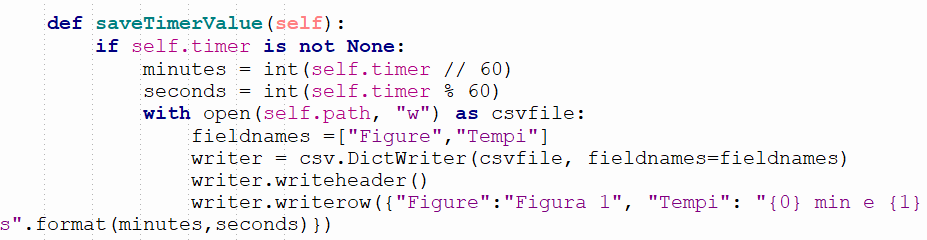
\includegraphics[width=1.15\textwidth]{immagini/stv.png}
\end{figure}
\vspace{0.4cm}
\end{itemize}
}
\newpage
\section{Risultati e obiettivi raggiunti}
\fontsize{12}{19}\selectfont{Questa sezione offre l'opportunità di riepilogare ed analizzare i principali risultati ottenuti e di sottolineare l'allineamento tra gli obiettivi prefissati e quelli raggiunti.\newline

Considerando i due test analizzati in precedenza, nel caso del \textbf{test sulla Discriminazione uditiva} si è sviluppata una applicazione
con comportamenti personalizzati del robot in grado di simulare la
somministrazione della prova da parte di un terapista.\newline
\begin{figure}[H]
\centering
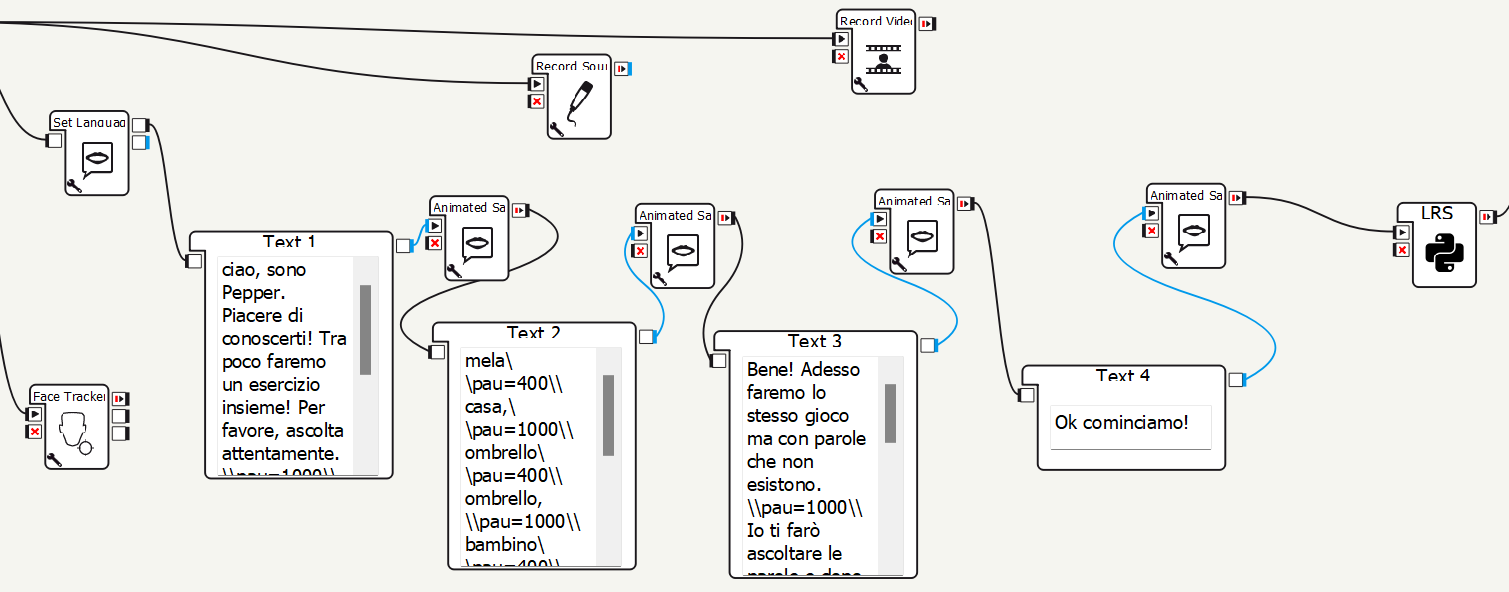
\includegraphics[width=1.1\textwidth]{immagini/tdu.png}
\caption{Panoramica sul test della Discriminazione uditiva}
\end{figure}
\vspace{0.4cm}
Più nello specifico,
inizialmente Pepper effettua un’ introduzione al test, spiegando dettagliatamente
le regole di quest’ultimo, per poi comunicare al paziente le 37 coppie
di \textit{non parole}.\newline
Il robot attende la risposta del paziente e aggiorna il suo
score prima di aver comunicato la successiva coppia di non parole. Al termine
del test si è in grado di visionare un file di testo contente lo \textit{score} del paziente,
da analizzare successivamente.\newline

Analizzando invece il \textbf{test della Torre di Londra (ToL)}, l’applicazione
sviluppata permette anche in questo caso di simulare la somministrazione
della prova da parte di un terapista, pur non sostituendo la sua valutazione.\newline
Il robot dopo una prima fase nella quale fornisce al paziente una spiegazione
delle regole, mostra una configurazione di prova da utilizzare per verificare
la comprensione della struttura del test somministrandolo successivamente.
\vspace{0.6cm}
\begin{figure}[H]
\centering
\includegraphics[width=0.75\textwidth]{immagini/TOL1.png}
\caption{Esempio di configurazione che il paziente deve replicare (ToL)}
\end{figure}
\newpage
A questo punto il paziente visualizza sul tablet di Pepper la configurazione
da replicare, riproduce quella compresa e prosegue in questo modo fino ad
esaurire tutte le configurazioni fornite dall’umanoide.

Al termine della prova, verranno analizzati dal terapista tutti i dati raccolti, salvati nel file cvs realizzato da Pepper e contenente i tempi di esecuzione del paziente per ogni singola configurazione.
\vspace{0.6cm}
\begin{figure}[H]
\centering
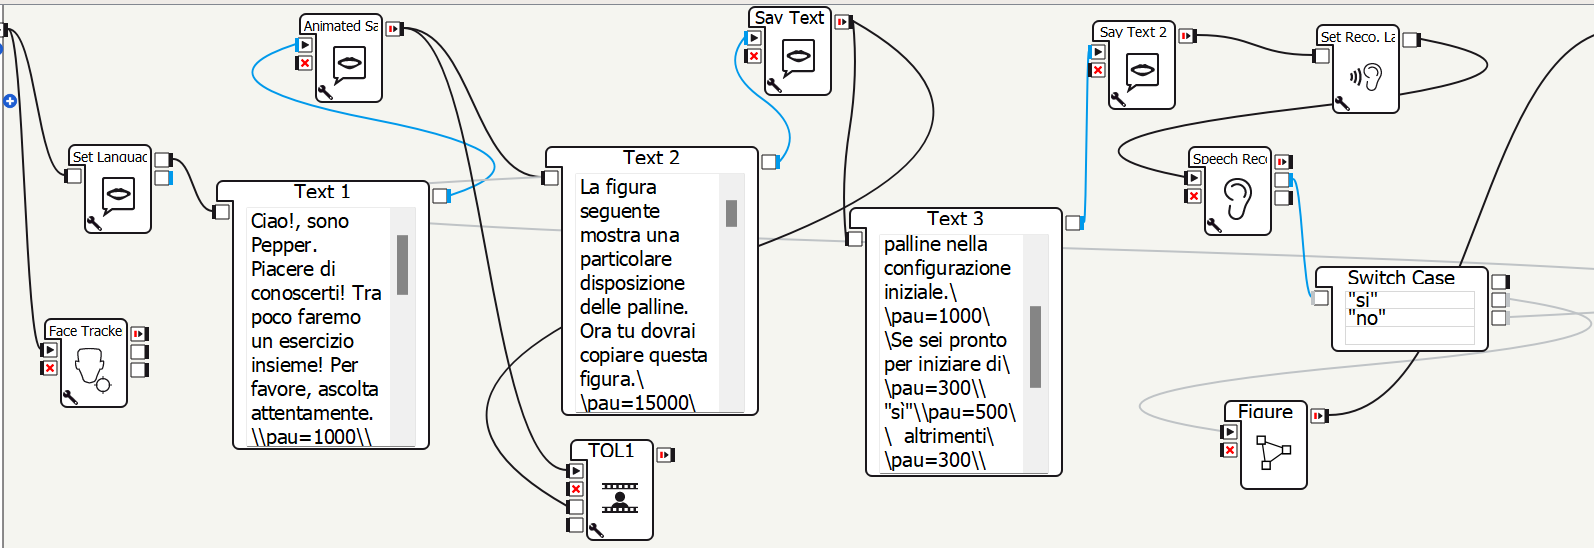
\includegraphics[width=1\textwidth]{immagini/tol1.png}
\caption{Panoramica sul test della Torre di Londra (ToL)}
\end{figure}
\vspace{1cm}
\begin{figure}[H]
\centering
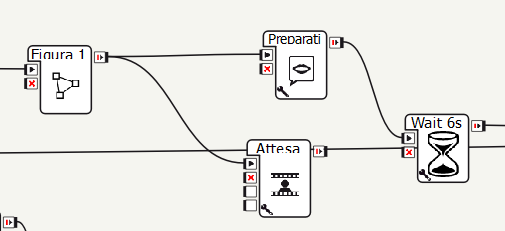
\includegraphics[width=0.7\textwidth]{immagini/tol2.png}
\caption{Implementazione della visualizzazione delle figure sul tablet di Pepper}
\end{figure}
\newpage
}
 \end{sloppypar}
\afterpage{\blankpage}